\subsection{Combining Spatial Enhancement Methods}
Når vi har brug for at forbedre et billede er det sjældent nok bare at bruge én methode. I stedet vil man anvenden en række filtre eller methode til at trække de relevante detaljer ud. Eksemplet fra bogen bruger røntgenbillede som object og anvender følgende methode i rækkefølge for at forbedre billedet til videre arbejde. 

\begin{enumerate}[(a)]
	\item \textbf{Originalbillede.}\label{a}\\
	Billedet som vi vil forbedre.
	
	\item \textbf{Laplacian af \ref{a}.}\label{b}\\
	Trække de fine detaljer ud, men er ellers bare grå og utydelig.
		
	\item \textbf{Lagt original~\ref{a} og Laplacian~\ref{b} sammen.}\label{c}\\
	Bruges for at highlighte de fine detaljer.

	\item \textbf{Sobel gradient fundet af original~\ref{a}.}\label{d}\\
	Gør kanterne skarpere.

	\item \textbf{Sobel billede \textit{smoothed} med 5 x 5 \textit{averaging filter}.}\label{e}\\
	Fundet med henblik på at tage produktet af \ref{d} (forrige) og \ref{e} (denne).

	\item \textbf{Maske fundet ved produkt af \ref{d} og \ref{e}.}\label{f}\\
	Lavet for at tage summen af \ref{a} og \ref{f} (denne).

	\item \textbf{Sharpened billede fundet ved sum af \ref{a} og \ref{f}.}\label{g}\\
	Fundet ved summen af \ref{a} og \ref{f}.

	\item \textbf{Endeligt resultat fundet ved at bruge \textit{power-law transformation} på \ref{g}.}\label{h}\\
	Resulterende billede.	
\end{enumerate}

Figur~\ref{fig:combined} viser orignalbilledet og resultatet.

\begin{figure}[H]
	\centering
	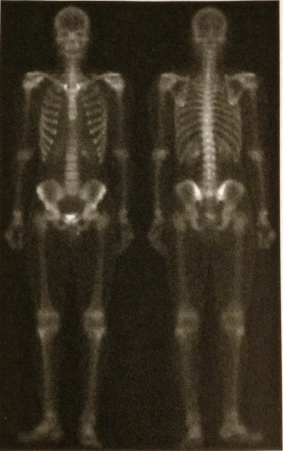
\includegraphics[width=0.4\linewidth]{figs/spm02/combinedfirst} \hfill
	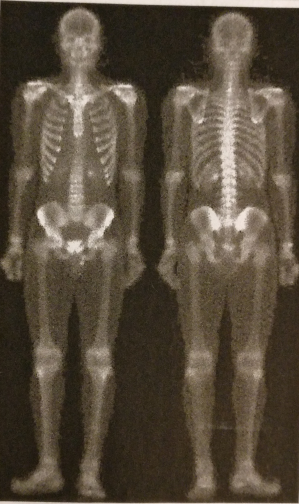
\includegraphics[width=0.4\linewidth]{figs/spm02/combinedlast}	
	\caption{Venstre: Det originale billede. Højre: Det resulterende billede.}
	\label{fig:combined}
\end{figure}
